% =============================================================================
% Paste-ready TikZ/PGFPlots figures for "Scale-Liberated StereoINR"
% Required preamble in main.tex (already present in the uploaded paper):
%   \usepackage{tikz,pgfplots}
%   \usetikzlibrary{arrows.meta,positioning,calc}
%   \pgfplotsset{compat=1.16}
%
% Every number below was checked against main.tex (Tables I-III, Sec. IV-V).
% Figures are vector graphics: no PNG, white background, paper-matched fonts.
% Labels fig:loss and fig:arch already exist in main.tex: when pasting Fig. 5
% and Fig. 6 below, REPLACE the existing figure environments, do not duplicate.
% =============================================================================

% ---------------------------------------------------------------------------
% FIGURE A (Pareto): Crop PSNR vs. latency, log x-axis, 90 Hz budget region
% Data: Table II (Crop PSNR means), Table I (latency). Measured points only.
% The foveated 256x256 tile is NOT plotted: its PSNR was never measured.
% ---------------------------------------------------------------------------
\begin{figure}[t]
\centering
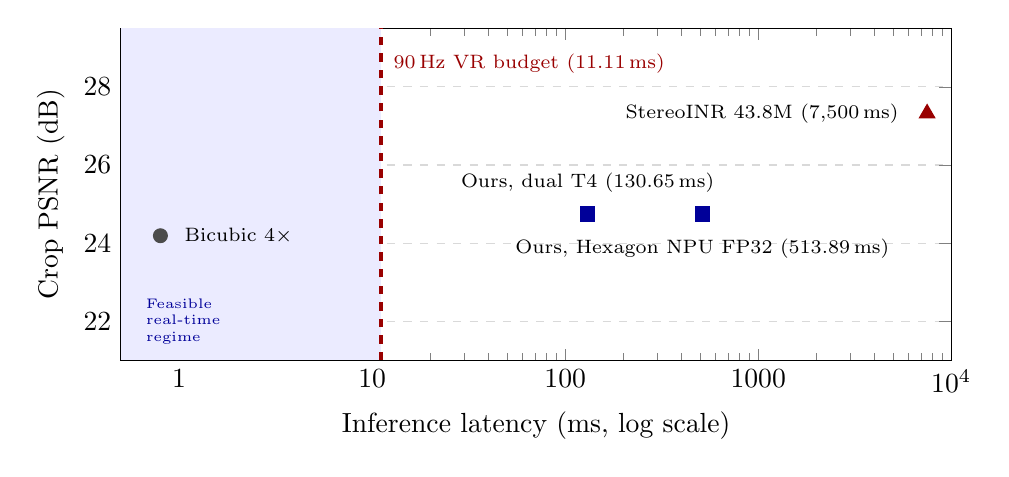
\begin{tikzpicture}
\begin{axis}[
    width=\columnwidth, height=5.8cm,
    xmode=log, xmin=0.5, xmax=10000, ymin=21, ymax=29.5,
    xtick={1,10,100,1000,10000}, xticklabels={1,10,100,1000,$10^4$},
    xlabel={Inference latency (ms, log scale)},
    ylabel={Crop PSNR (dB)},
    ymajorgrids, grid style={dashed, gray!30},
]
% Feasible real-time regime (x <= 11.11 ms)
\fill[blue!8] (axis cs:0.5,21) rectangle (axis cs:11.11,29.5);
% 90 Hz VR budget line
\draw[dashed, very thick, red!60!black] (axis cs:11.11,21) -- (axis cs:11.11,29.5);

\addplot[only marks, mark=*, mark size=2.5pt, gray!60!black]
    coordinates {(0.80,24.19)};
\addplot[only marks, mark=square*, mark size=2.6pt, blue!60!black]
    coordinates {(130.65,24.74) (513.89,24.74)};
\addplot[only marks, mark=triangle*, mark size=3.2pt, red!60!black]
    coordinates {(7500,27.32)};

\node[font=\scriptsize, anchor=west] at (axis cs:0.95,24.19) {Bicubic $4\times$};
\node[font=\scriptsize, anchor=south] at (axis cs:130.65,25.05) {Ours, dual T4 (130.65\,ms)};
\node[font=\scriptsize, anchor=north] at (axis cs:513.89,24.35) {Ours, Hexagon NPU FP32 (513.89\,ms)};
\node[font=\scriptsize, anchor=east] at (axis cs:6000,27.32) {StereoINR 43.8M (7{,}500\,ms)};
\node[font=\scriptsize, anchor=west, red!60!black] at (axis cs:11.5,28.6) {90\,Hz VR budget (11.11\,ms)};
\node[font=\tiny, anchor=west, align=left, blue!60!black] at (axis cs:0.6,22.0) {Feasible\\real-time\\regime};
\end{axis}
\end{tikzpicture}
\caption{Quality--latency trade-off on the 15-scene crop benchmark ($\times 4$, $128\times128$ crops; mean Crop PSNR). StereoINR reaches higher PSNR (27.32\,dB) but takes 7{,}500\,ms, $675\times$ the 11.11\,ms 90\,Hz budget. Our full-frame model reduces latency by $57.4\times$ (130.65\,ms on dual T4) and is $11.8\times$ above budget at full frame (46$\times$ for NPU FP32), so foveated execution is required to meet the 90\,Hz constraint. The NPU point reuses the mean PSNR of the same FP32 model, which is an assumption to state in the text.}
\label{fig:pareto}
\end{figure}

% ---------------------------------------------------------------------------
% FIGURE B (Latency budget): horizontal log-scale bars vs. 11.11 ms budget
% Data: Table I + Sec. IV-B (4.20 ms foveated NPU tile, 513.89 ms NPU FP32).
% ---------------------------------------------------------------------------
\begin{figure}[t]
\centering
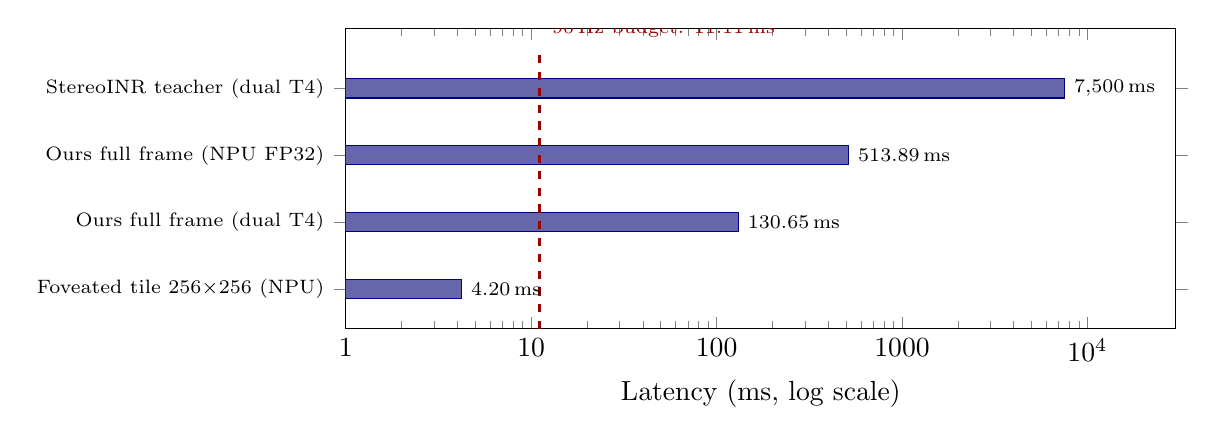
\begin{tikzpicture}
\begin{axis}[
    xbar, xmode=log, xmin=1, xmax=30000,
    width=\columnwidth, height=5.4cm, bar width=7pt,
    ytick={0,1,2,3},
    yticklabels={Foveated tile $256{\times}256$ (NPU),
                 Ours full frame (dual T4),
                 Ours full frame (NPU FP32),
                 StereoINR teacher (dual T4)},
    y tick label style={font=\scriptsize, align=right},
    xtick={1,10,100,1000,10000}, xticklabels={1,10,100,1000,$10^4$},
    xlabel={Latency (ms, log scale)},
    ymin=-0.6, ymax=3.9,
    enlarge y limits=false,
    nodes near coords,
    every node near coord/.append style={font=\scriptsize, anchor=west},
    point meta=explicit symbolic,
]
\addplot[fill=blue!45!black!60, draw=blue!50!black]
    coordinates {(4.20,0) [4.20\,ms] (130.65,1) [130.65\,ms]
                 (513.89,2) [513.89\,ms] (7500,3) [7{,}500\,ms]};
% 90 Hz budget marker
\draw[dashed, very thick, red!60!black] (axis cs:11.11,-0.6) -- (axis cs:11.11,3.6);
\node[font=\scriptsize, anchor=south west, red!60!black] at (axis cs:11.5,3.62)
    {90\,Hz budget: 11.11\,ms};
\end{axis}
\end{tikzpicture}
\caption{End-to-end latency against the Quest~3S 90\,Hz budget (11.11\,ms, dashed). Only the $256{\times}256$ foveal tile on the Hexagon NPU (4.20\,ms) fits the budget. Full-frame inference takes 130.65\,ms on dual T4 and 513.89\,ms in FP32 on the NPU (358.64\,ms INT8, Table I).}
\label{fig:latency}
\end{figure}

% ---------------------------------------------------------------------------
% FIGURE C (Memory access schematic). Schematic, not a measurement: the
% manuscript reports no cache hit rates, so none are shown.
% ---------------------------------------------------------------------------
\begin{figure*}[t]
\centering
\begin{tikzpicture}[>={Stealth[length=2mm]}, font=\small]
% (a) StereoINR: scattered 2D sampling over a 6x6 feature grid
\begin{scope}
\node[font=\small\bfseries] at (1.5,3.4) {(a) StereoINR: unconstrained 2D deformable sampling};
\foreach \i in {0,...,5} \foreach \j in {0,...,5}
    \draw[gray!50] (\i*0.5,\j*0.5) rectangle (\i*0.5+0.5,\j*0.5+0.5);
\draw[red!70!black, thick, ->] (0.25,0.25) -- (2.25,1.75);
\draw[red!70!black, thick, ->] (2.75,0.25) -- (0.75,2.25);
\draw[red!70!black, thick, ->] (0.25,2.75) -- (2.75,2.25);
\draw[red!70!black, thick, ->] (1.25,0.75) -- (2.75,2.75);
\draw[red!70!black, thick, ->] (2.25,2.75) -- (0.25,0.75);
\node[font=\scriptsize, text=red!60!black, align=center] at (1.5,-0.5)
    {Random DRAM strides, scattered row crossings\\(non-contiguous reads)};
\end{scope}

% (b) Ours: EPA-1D contiguous scanline bursts
\begin{scope}[shift={(7,0)}]
\node[font=\small\bfseries] at (1.5,3.4) {(b) Ours: EPA-1D scanline attention};
\foreach \i in {0,...,7} \draw[gray!50] (\i*0.375,2.2) rectangle (\i*0.375+0.375,2.575);
\draw[green!40!black, ultra thick, ->] (0.05,1.9) -- (1.45,1.9);
\draw[green!40!black, ultra thick, ->] (1.55,1.9) -- (2.95,1.9);
\draw[green!40!black, ultra thick, ->] (0.05,1.35) -- (2.95,1.35);
\node[font=\scriptsize, text=green!40!black, align=center] at (1.5,0.6)
    {Contiguous 1D burst reads along the epipolar scanline};
\end{scope}

% Comparison table
\node at (4.25,-2.2) {%
\begin{tabular}{@{}lll@{}}
\toprule
\textbf{Property} & \textbf{StereoINR (official)} & \textbf{Ours (EPA-1D)} \\
\midrule
Memory access pattern & Scattered 2D & Contiguous 1D \\
Qualcomm Hexagon NPU & Compilation rejected (\texttt{GridSample}) & 100\% native NPU (1,495/1,495 ops, 0\% CPU fallback) \\
\bottomrule
\end{tabular}};
\end{tikzpicture}
\caption{Memory-access and operator-level comparison. Panel (a) and (b) are schematics of the access pattern; Table below lists the measured compilation outcomes reported in Sec.~IV-B.}
\label{fig:memaccess}
\end{figure*}

% ---------------------------------------------------------------------------
% FIGURE D (NPU compilation and hardware profile). Formal table.
% All values from Table I and Sec. IV-B of main.tex.
% ---------------------------------------------------------------------------
\begin{figure}[t]
\centering
\small
\begin{tabular}{@{}lll@{}}
\toprule
\textbf{Metric} & \textbf{StereoINR (official)} & \textbf{Ours} \\
\midrule
Parameters & 43{,}791{,}595 & 4{,}468{,}180 \\
INT8 model size & 41.8~MB & 4.26~MB \\
Qualcomm NPU compilation & Rejected (\texttt{GridSample}) & 100\% native (QNN DLC) \\
NPU operator coverage & -- & 1,495/1,495 (0\% CPU fallback) \\
Peak VRAM (dual T4) & 1{,}840~MB & 426~MB \\
Peak NPU memory & -- & 77.29~MB \\
Latency, dual T4 (full frame) & 7{,}500.00~ms & 130.65~ms \\
Latency, NPU FP32 (full frame) & -- & 513.89~ms \\
Latency, NPU INT8 (full frame) & -- & 358.64~ms \\
Latency, NPU foveated $256{\times}256$ & -- & 4.20~ms \\
\bottomrule
\end{tabular}
\caption{Qualcomm Hexagon NPU compilation and hardware profile (dual Tesla T4 for GPU rows; Qualcomm AI Hub profile for NPU rows). ``--'' means not reported in the manuscript.}
\label{fig:npu_profile}
\end{figure}

% ---------------------------------------------------------------------------
% FIGURE E (Training loss). Only the TOTAL loss per epoch exists in the
% manuscript data. Per-component curves are not included because no
% per-epoch component values are available. Do not add them without logs.
% ---------------------------------------------------------------------------
\begin{figure}[t]
\centering
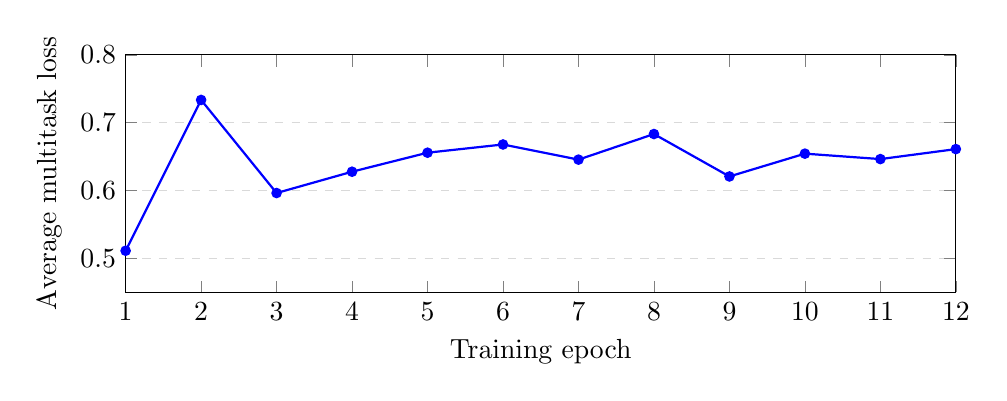
\begin{tikzpicture}
\begin{axis}[
    width=\columnwidth, height=4.6cm,
    xlabel={Training epoch}, ylabel={Average multitask loss},
    xmin=1, xmax=12, ymin=0.45, ymax=0.80,
    xtick={1,2,3,4,5,6,7,8,9,10,11,12},
    ymajorgrids, grid style={dashed, gray!30},
]
\addplot[blue, mark=*, mark size=1.5pt, thick] coordinates {
    (1,0.5114) (2,0.7335) (3,0.5964) (4,0.6278) (5,0.6558) (6,0.6679)
    (7,0.6456) (8,0.6833) (9,0.6208) (10,0.6544) (11,0.6464) (12,0.6611)
};
\end{axis}
\end{tikzpicture}
\caption{Total multitask training loss per epoch (12 epochs, 84 steps, dual Tesla T4 DDP, 86.9\,s). The brief schedule is an under-trained regime, which accounts for part of the capacity gap to the 43.8M teacher.}
\label{fig:loss}
\end{figure}

% ---------------------------------------------------------------------------
% FIGURE F (Foveated pipeline). Quest 3S has no eye tracker (Sec. VI-2),
% so the tile is fixed at the optical centre. Gaze input is NOT drawn.
% ---------------------------------------------------------------------------
\begin{figure*}[t]
\centering
\begin{tikzpicture}[
    >={Stealth[length=2mm]},
    box/.style={draw, rounded corners=2pt, align=center, font=\small,
                minimum height=1.1cm, text width=3.3cm, fill=gray!5}]
\node[box] (a) {Fixed central\\$256{\times}256$ tile\\(optical centre)};
\node[box, right=1.0cm of a] (b) {EPA-1D inference\\on Hexagon NPU\\(4.20\,ms)};
\node[box, right=1.0cm of b] (c) {Radial Hann\\$\alpha$-blend};
\node[box, right=1.0cm of c] (d) {Display\\framebuffer};
\draw[->, thick] (a) -- (b);
\draw[->, thick] (b) -- (c);
\draw[->, thick] (c) -- (d);
\end{tikzpicture}
\caption{Foveated passthrough pipeline. Quest~3S has no eye-tracking cameras, so the super-resolved tile is fixed to the optical centre (Sec.~VI-2). The Hann blend weight is given in Fig.~\ref{fig:hann}.}
\label{fig:foveated}
\end{figure*}

% ---------------------------------------------------------------------------
% FIGURE G (Hann blending weight). Corrected: alpha = 1 at the fovea (r_in)
% and 0 at the outer radius (r_out). The prompt's sign was inverted.
% ---------------------------------------------------------------------------
\begin{figure}[t]
\centering
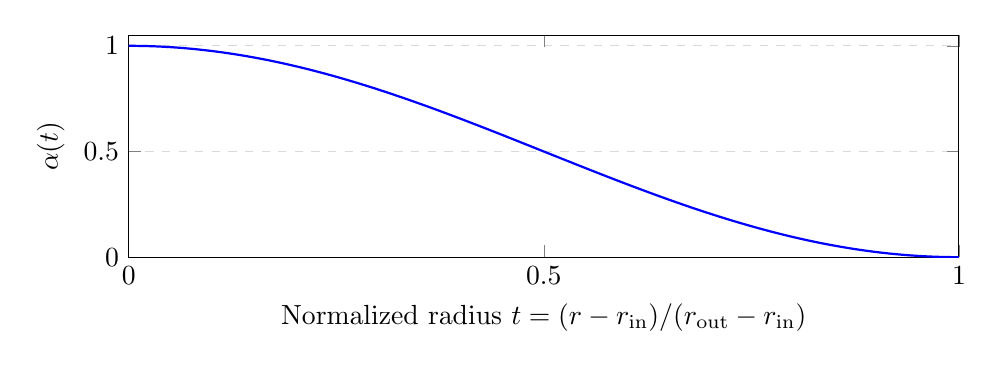
\begin{tikzpicture}
\begin{axis}[
    width=\columnwidth, height=4.4cm,
    xmin=0, xmax=1, ymin=0, ymax=1.05,
    xlabel={Normalized radius $t=(r-r_{\mathrm{in}})/(r_{\mathrm{out}}-r_{\mathrm{in}})$},
    ylabel={$\alpha(t)$},
    xtick={0,0.5,1}, ytick={0,0.5,1},
    ymajorgrids, grid style={dashed, gray!30},
]
\addplot[blue, thick, domain=0:1, samples=120] {0.5+0.5*cos(180*x)};
\end{axis}
\end{tikzpicture}
\caption{Radial Hann blending weight $\alpha(r)=0.5+0.5\cos\!\big(\pi\,\frac{r-r_{\mathrm{in}}}{r_{\mathrm{out}}-r_{\mathrm{in}}}\big)$ for $r_{\mathrm{in}}\le r\le r_{\mathrm{out}}$: $\alpha=1$ at the fovea and $\alpha=0$ at the outer radius, giving a smooth transition.}
\label{fig:hann}
\end{figure}
